\documentclass[a4paper]{article}

\usepackage[utf8]{inputenc}   
\usepackage[T1]{fontenc}      
\usepackage[francais]{babel}  

\usepackage{url}
\usepackage{listings}
\lstset{language=python} % more options are welcome, RTFM!

\usepackage{graphicx}
\usepackage[marginpar]{todo}

\usepackage[a4paper]{geometry}

\title{Pythran : Rapport court}           
\author{Alan Raynaud}
\date{}                      

\sloppy 

\begin{document}

%Page de garde

\maketitle   
\begin{abstract}
    trop de la balouze ce sujet\todo{Ecrire un résumé plus explicite.}
\end{abstract}

\clearpage               

\tableofcontents            

\clearpage

\section{Analyse bibliographique}             

\subsection{Introduction : du Python et des performances}

Python, langage interprété et dynamiquement typé, est la plupart du
temps moins performant que d'autres langages compilés comme C ou
C++\cite{PythonVsCpp}. On se contente souvent de définir la
performance d'un programme comme étant sa vitesse d'exécution par
rapport à un programme semblabme écrit dans un langage différent ou
utilisant un autre algorithme. C'est cette définition restreinte qui
sera utilisée sous le nom de performance dans la suite\footnote{Il
  existe de nombreux travaux sur la manière de mesurer scentifiquement
  la performance d'un programme, qui s'appuient sur de nombreux
  indicateurs en plus du temps d'exécution. L'un des spécialiste du
  domaine résume cela de manière informelle en ces mots : "The word
  performance in computer performance means the same thing that
  performance means in other contexts, that is, it means 'How well is
  the computer doing the work it is supposed to
  do?'"\cite{Allen}}. Toutes les applications n'ont pas un même besoin
en performances, et celles du Python sont généralement considérées
comme suffisantes dans la plupart des cas. Il existe cependant des
applications qui effectuent des calculs intensifs ou doivent traiter
de très grande quantités de données, et qui ont donc besoin que
certains de leurs algorithmes soient effectués avec des performances
supérieures à celles ordinairement obtenues avec Python.

\subsection{Utilisation d'un Python plus performant}

\label{OptCode}

\subsubsection{Bonne pratiques de codage}

Un des principes de la philosophie python est ``There should be one--
and preferably only one --obvious way to do it.''\cite{ZenPython} Le
souci d'optimiser les performances d'un programme python induit
cependant plus de reflexions quant à la manière de résoudre un
problème. C'est pour cela qu'il existe des guides donnant bonnes
pratique pour écrire un programme python le plus performant
possible\cite{PythonSpeed}.

Exemples :
\begin{itemize}
\item Concaténer des strings avec .join() plutôt qu'avec l'opérateur +.
\item Utiliser plusieurs affectations plutôt qu'une affectation
  multiple : \lstinline|a=x;b=y;| plutôt que \lstinline|a,b=x,y|.
\item Utiliser les opérateurs propres au langage plutôt que les
  fonctions lambda : \lstinline|operator.add| plutôt que
  \lstinline|lambda x,y : x+y|.
\end{itemize}

\subsubsection{Itérateurs et générateur}

Dans la boucle de l'exemple suivant, Python génère la liste [1..100]
puis créé un objet itérateur qui permet de parcourir un à un les
éléments de cette liste.

\begin{lstlisting}
for i in range(100):
  print i
\end{lstlisting}

On se rend compte dans cet exemple qu'il n'était pas nécessaire
d'avoir toute la liste en mémoire. En effet, un seul élément est
utilisé à la fois, et chaque élément n'est utilisé qu'une seule fois.

C'est pourquoi il existe en Python des générateurs. Les générateurs
permettent de réaliser des itérateurs qui ne parcourent pas un
ensemble, mais génèrent les éléments de l'itération au fur et à
mesure. Quand on utilise un itérateur produit par un générateur, il
n'y a toujours qu'une seule valeur en mémoire : celle actuellement
utilisée.

Python fournit également des itérateurs se comportant comme ceux
produits par des générateurs :

\begin{itemize}
\item \texttt{xrange} qui se comporte comme \texttt{range}, mais ne
  créé pas de liste en mémoire.
\item les itérateurs du module \texttt{itertools} comme \texttt{imap}
  et \texttt{product}.
\end{itemize}

Afin de considérer l'intérêt en terme de performances, on peut
considérer la figure~\ref{GenExpMapImapPy}, qui montre les différences
de temps d'exécution entre trois implémentations du calcul de la somme
des carrés des N premiers entiers.

\begin{figure}[h]
  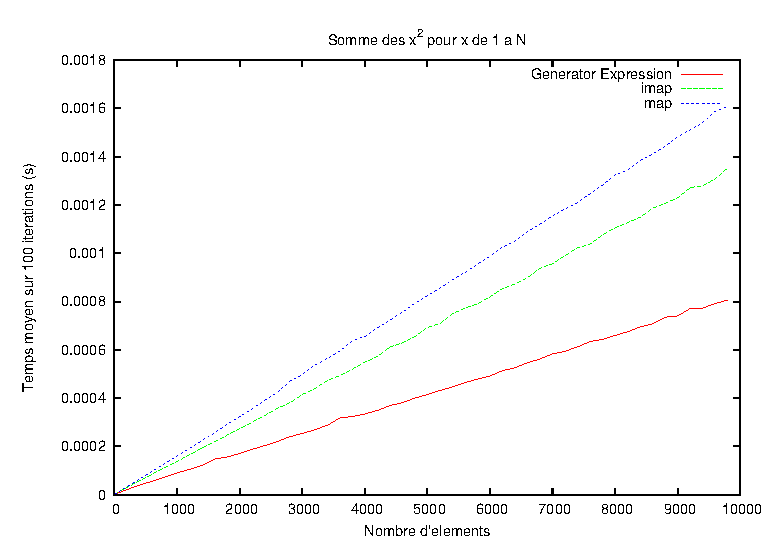
\includegraphics[width=\textwidth]{./Pictures/GenExpMapImapPy}
  \caption{Comparaison de performances entre trois implémentations en Python.}
  \label{GenExpMapImapPy}
\end{figure}

Les évaluations de performances sont effectuées sur une machine
comportant un processeur de type Intel Core i3 4G de RAM, un noyau
Linux 3.2.0 et python 2.7.3.  Dans chaque cas, le temps de l'exécution
de 100 itérations du même programme est mesuré grâce au module
\texttt{timeit}. Le module \texttt{timeit} est un module de python
fournissant des outils pour mesures les temps d'exécution de morceaux
de code python. En particulier, la fonction
\lstinline|timeit.timeit(expr, number = n)| permet de mesurer le temps
de n executions du code contenu dans \texttt{expr}.

\begin{lstlisting}
time100 = timeit.timeit('Expression', number=100)
\end{lstlisting}

La première implémentation utilise un générateur :

\begin{lstlisting}
sum(x*x for x in xrange(N))
\end{lstlisting}

Le générateur créé permet de ne produire les carrés qu'au fur et à
mesure de la sommation. À un instant donné, il n'y a qu'un seul carré
en mémoire.

La seconde implémentation utilise la fonction \texttt{imap} qui
applique une fonction à un itérateur pour produire un nouvel
itérateur~:

\begin{lstlisting}
sum(imap(lambda x:x*x, xrange(N)))
\end{lstlisting}

Cette implémentation est moins performante que la première car elle
utilise des appels de fonction, qui sont coûteux en
Python.\todo{argumenter}

La troisième implémentation utilise la fonction \texttt{map} qui
applique une fonction à un itérateur pour produire une liste :

\begin{lstlisting}
sum(map(lambda x:x*x, xrange(N)))
\end{lstlisting}

Dans cette implémentation, la liste des carrés est créée avant la
sommation. C'est l'opération de création de l'espace mémoire
nécessaire pour la stocker qui est coûteuse et diminue les performance
par rapport à la seconde implémentation.

On remarque bien que l'implémentation choisie peut faire
considérablement varier le temps d'exécution. On constate également
que le simple fait de remplacer \texttt{map} par \texttt{imap} permet
un gain de performance non négligeable dès que l'on manipule un large
ensemble de données. La même constatation peut être faite quand à
l'utilisation de \texttt{xrange} plutôt que \texttt{range} ou encore
\texttt{izip} plutôt que \texttt{zip}.\todo{pour plus atrd: comment
  mesurer l'utilisation émmoire et la comparer?}

\subsubsection{Module spécialisés}

Il existe des modules pour Python destinés à permettre de réaliser des
applications de calcul scientifiques en Python.  C'est par exemple le
cas du package NumPy, qui fournit à Python des fonctionnalités proches
de celles de matlab. Les modules de numpy sont écrit en C, de façon à
permettre à un programme les utilisant d'avoir des performances
proches d'un programme écrit en C\cite{NumPyPerf}.

\subsection{Optimisation à partir du code Python}

Les méthodes d'amélioration des performances présentées en
\ref{OptCode} nécessitent d'effectuer des modifications au niveau du
code source. Les gains en temps d'exécution se feront donc au prix
d'une augmentation du temps de développement. Il existe cependant des
outils qui permettent d'augmenter les performances d'un programme sans
avoir à modifier le code source.

\subsubsection{Optimisation de l'interpréteur}

CPython est l'implémentation de référence du langage Python. Il en
existe cependant d'autre comme Jython écrit en Java et IronPython,
l'implémentation de Python pour .NET. Le projet Pypy, quant à lui, a
pour but d'obtenir une implémentation de Python plus performante que
CPython.

Un programme écrit en Python pour CPython peut être exécuté avec Pypy
sans modification\footnote{Il existe quelques incompatibilités dans
  des cas particuliers, souvent liées à des différence de stratégie
  des ramasse-miettes\cite{PypyDiff}.} et sera en moyenne 5,5 fois
plus rapide\cite{PypySpeed}.

\subsubsection{La solution pythran : compiler en code natif}

L'outils pythran permet de traduire un module Python en C++ pour
pouvoir ensuite être compilé en code natif. Afin d'être utilisable par
pythran, le code source doit seulement être annoté de descriptions
d'interfaces. Le résultat est un module Python en code natif qui peut
être utilisé depuis un programme Python usuel. Pythran ne traduit
qu'un sous-ensemble de Python. En particulier, les classes ne sont pas
gérées. Cela destine pythran à être utilisé pour l'optimisation
d'algorithmes dont les temps d'exécution sont critiques pour le
programme les utilisant.

La figure~\ref{RangeXrangePyCpp} permet de comparer les performances
entre un programme en Python et son équivalent en C++.

\begin{figure}[h]
  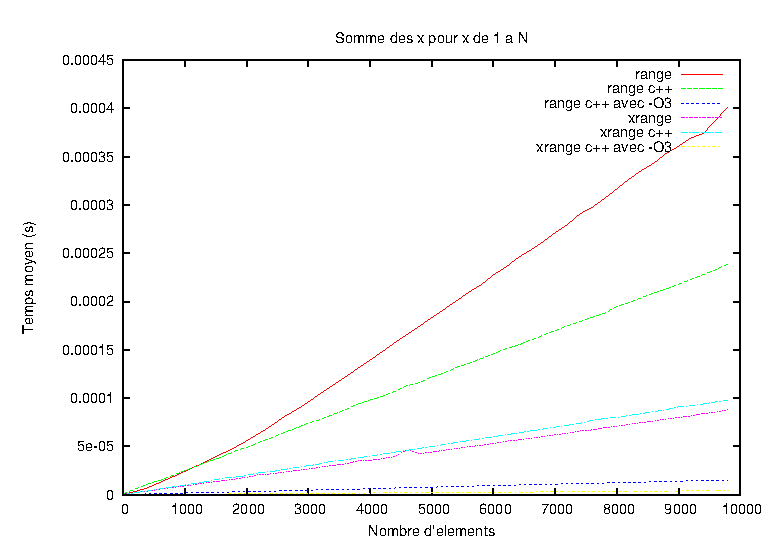
\includegraphics[width=\textwidth]{./Pictures/RangeXrangePyCpp}
  \caption{Comparaison de performances entre Python et C++ compilé
    avec et sans le flag -O3.}
  \label{RangeXrangePyCpp}
\end{figure}

Les programme en Python sont les suivants :

\begin{lstlisting}
  sum(range(N))
\end{lstlisting}

\begin{lstlisting}
  sum(xrange(N))
\end{lstlisting}

et leurs équivalents en C++ sont :

\begin{lstlisting}
  pythonic::sum(pythonic::range(N))
\end{lstlisting}

\begin{lstlisting}
  pythonic::sum(pythonic::xrange(N))
\end{lstlisting}

où \texttt{pythonic} est le namespace de Pythonic++ (cf. \ref{Pythonicpp}
p. \pageref{Pythonicpp}).

Les temps en Python sont de nouveau mesurés avec \texttt{timeit.timeit()} et
les temps en C++ sont mesurés avec \texttt{clock()}.

\begin{figure}[h]
  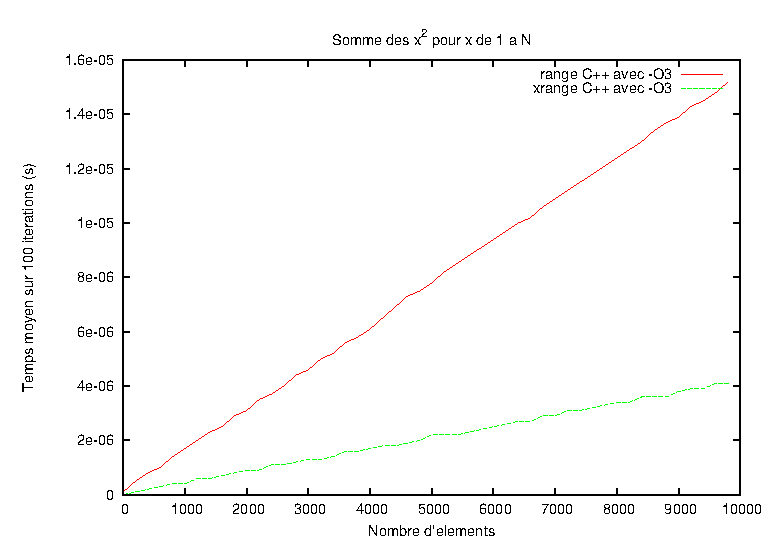
\includegraphics[width=\textwidth]{./Pictures/RangeXrangeCppO3}
  \caption{Comparaison entre \texttt{range} et \texttt{xrange} en C++
    avec le drapeau -O3.}
  \label{RangeXrangeCppO3}
\end{figure}

On remarque que, contrairement à ce à quoi on pouvait s'attendre, les
implémentations en C++ ne sont pas toujours plus rapides que celles en
Python. Dans le cas du \texttt{xrange}, le programme en Python est
légèrement plus performant que celui en C++. Cependant, l'optimisation
du compilateur C++ permet de réduire de façon drastique le temps
d'exécution. Enfin, le gain réalisé en remplaçant \texttt{range} par
\texttt{xrange} se retrouve également en C++, comme le montre la
figure~\ref{RangeXrangeCppO3}.

De cela on peut en conclure que pythran peut augmenter les
performances d'un algorithme sur trois axes :

\begin{itemize}
\item Optimisation du code d'origine, par exemple en remplaçant
  automatiquement des fonctions comme \texttt{range} ou \texttt{map}
  par \texttt{xrange} et \texttt{imap}.
\item Traduction en code C++ pour pouvoir être compilé en code natif,
  en général plus rapide que du code interprété.
\item Possibilité de bénéficier des optimisations supplémentaires du
  compilateur C++.
\end{itemize}


Pythran permet également d'annoter le programme de directives OpenMP,
qui permettent de paralléliser les opérations qui peuvent l'être. Cela
nécessite une analyse du programme pour déterminer les opérations
parallélisables, mais cela permet d'augmenter encore la vitesse
d'exécution d'un facteur x2 à x4\cite{PythranRenpar}.

\section{Analyse du problème}

Le code Python lu par pythran est représenté sous forme d'un arbre
syntaxique abstrait (AST) dont les noeuds représentent des opérateurs
et les feuilles des opérandes. C'est sur cet arbre que pythran
travaille pour optimiser le programme et le traduire en C++.

\subsection{Transformations de l'AST}

Avant de produire la traduction C++, pythran peut effectuer des
opérations sur l'AST. Ces opérations visent à apporter des
modifications ne changeant pas les résultats produits par le
programme, mais utilisant des combinaisons d'opérateurs plus
performantes celles initialement utilisées. On appelle ce type de
modification une transformation de l'AST.

\subsubsection{Recherche de transformations valide}

La recherche de transformations pertinentes nécessitent d'avoir des
connaissance pointues sur le coût des différentes opérations
effectuées par un même opérateur. Par exemple, c'est parce que
l'allocation d'une grande quantité de mémoire a un coût prohibitif que
les transformation du type \texttt{range} -> \texttt{xrange}
permettent un gain de performances.

Un autre problème est celui de la recherche de la validité d'une
transformation. On a vu qu'une transformation consiste à remplacer une
combinaison d'opérateurs par une autre combinaison équivalente. Or,
cette équivalence peut n'être vérifiée que sous certaines
conditions. La transformation n'est alors valide que dans les cas où
ces conditions sont toutes vérifiées.

Dans le cas de \texttt{xrange}, une condition suffisante pour que la
transformation \texttt{range} -> \texttt{xrange} soit valide est que le résultat produit
par\texttt{range}ne soit jamais modifié. Ce qui serait par exemple le cas
dans l'exemple suivant\footnote{En supposant que range(100) soit bien
  une opération produisant la liste [1..100].} :

\begin{lstlisting}
  for i in range(100):
    f(i)
\end{lstlisting}

Ceci peut donc être remplacé par

\begin{lstlisting}
  for i in xrange(100):
    f(i)
\end{lstlisting}

\subsubsection{Le problème du contexte}

Un obstacle majeur est qu'il n'est pas trivial de savoir si les
conditions de validité de la transformation sont remplies.

Par exemple, il est possible d'appliquer la transformation \texttt{range} ->
\texttt{xrange} au programme suivant. Mais pour pouvoir savoir cela, il faut
vérifier le reste du code pour s'assurer que la liste assignée à la
variable l n'est jamais modifiée.

\begin{lstlisting}
  l = range(100)
  .
  .
  .
  for i in l:
    f(i)
\end{lstlisting}

Un autre problème vient du fait que dans l'AST, un opérateur est
représenté par son nom, ce qui permet la situation de l'exemple
suivant, où la transformation \texttt{range()} -> \texttt{xrange()} n'est pas valide
dans la boucle for.\todo{pas en gros problème, juste une gestion des portées... on a déjà l'analyse qui faut.Mais qui de foo(range(100))? a=range(18) ?}

\begin{lstlisting}
  def g(n):
    return [9001,n,27,42]
  .
  .
  .
  range = g
  .
  .
  .
  for i in range(100):
    f(i)
\end{lstlisting}

Avant d'effectuer la transformation, il faut donc analyser le
programme pour déterminer dans quels cas la transformation est
valide. Dans pythran, c'est ce que réalisent les analyses, qui
parcourent et annotent l'AST. Les transformations appliquées ensuite
utilisent les annotations laissées par les analyses.

Un exemple simple est celui de la réduction des expressions
constantes. Une analyse parcourt l'AST pour déterminer quels noeuds
correspondent à des expressions constantes. Une transformation peut
ensuite être appliquée à ces noeuds pour les réduire en feuille.

\subsection{Compilation du code optimisé}

\label{Pythonicpp}

C'est à partir de l'AST optimisé que pythran génère le code C++. Pour
cela, il utilise Pythonic++, un ensemble de headers C++ qui
contiennent les équivalents en C++ des opérateurs et des collections
natives au Python.

Pour qu'un module de la bibliothèque standard de Python puisse être
utilisé dans du code traduit par pythran, il faut donc qu'un
équivalent de ce module ai été développé pour Pythonic++. Ce n'est pas
encore le cas du module \texttt{itertools}, ce qui empêche d'utiliser des
fonctions comme \texttt{imap} ou \texttt{product}.

\section{Plan de travail}

L'ordre envisagé pour le plan de travail prend en compte plusieurs
paramètres :

\begin{itemize}
\item Certains travaux dépendent des résultats des autres. En
  particulier, la plupart des transformations de l'AST visent à
  utiliser des fonctions du module \texttt{itertools} dès que cela est
  possible. Ces transformations ne peuvent donc être implémentées
  qu'une fois le module \texttt{itertools} disponible dans Pythonic++.
\item Certains travaux sont plus simples et permettent d'assimiler les
  concepts et outils nécessaires à la réalisation des travaux plus
  complexes du même type. Par exemple, la transformation de
  \texttt{range} en \texttt{xrange} est complexe et devrait donc être
  abordée après que la transformation de generator expression en
  \texttt{imap} ait été complétée.
\end{itemize}

\subsection{Implémentation du module \texttt{Itertools}}

\subsubsection{Méthodologie}

La méthodologie utilisée pour l'implémentation du module \texttt{itertools} est
une itération des étapes suivantes :

\begin{enumerate}
\item Déterminer une fonction à implémenter.
\item Écrire des tests.
\item Implémenter la fonction en C++ dans Pythonic++.
\item Tester la fonction pour vérifier qu'elle produit le résultat
  attendu pour tout les cas de test.\todo{préciser que c'est fait
    automatiquement par la suite de test existante ? -> ah?}
  \item Tester les performances de la fonction et vérifier qu'il n'y a
    pas d'opération anormalement coûteuse avec le module CallGrind de
    l'outils Vallgrind.
\end{enumerate}

\subsubsection{Priorités}

Les opérateurs à implémenter en priorités sont ceux nécessaires à
l'implémentation des nouvelles transformations :

\begin{itemize}
  \item \texttt{imap}
  \item \texttt{product}
  \item \texttt{ifilter}
\end{itemize}


\subsection{Transformation de l'AST}

Une seconde partie du travail consistera à mettre au point des
transformations de l'AST pertinentes. En particulier, il faudra
déterminer dans quel cas elles sont valides et s'assurer de ne les
appliquer que dans ces cas.

\subsubsection{Les generator expressions}

En Python, les generator expression sont plus performantes que
l'utilisation de \texttt{map} ou \texttt{imap}. Cependant, cela est lié au coût
prohibitif d'un appel de fonction en Python. Une fois traduit en C++,
ce surcoût devrait être moindre et devrait rendre l'implémentation de
\texttt{imap} plus performante que l'équivalent des generator expressions.

Il sera alors pertinent de remplacer

\begin{lstlisting}
(g(a,b,c...) for a in A if fa(a) for b in B if fb(a,b) for c in C if fc(a,b,c) ... )
\end{lstlisting}
 
par

\begin{lstlisting}
imap(lambda a,b,c... : g(a,b,c...), 
  ifilter(lambda a,b,c... : fa(a) and fb(a,b) and fc(a,b,c)..., product(A,B,C...)))
\end{lstlisting}

Cette transformation est toujours valide et ne nécessitera pas
d'écrire une analyse. Il faudra donc simplement implémenter la
transformation, et effectuer des tests pour vérifier qu'elle apporte
bien un gain de performances après traduction en C++.

\subsubsection{Le cas \texttt{xrange}}

\todo{pas uniquement xrange: map ->imap, zip ->izip,[x for x..] ->(x for x...)}

Les exemples précédents ont montré que la transformation
\texttt{range} -> \texttt{xrange} n'est pas toujours valide. Il faudra
donc :

\begin{enumerate}
\item Identifier la plupart des cas dans lesquels la transformation
  est valide.
\item Écrire une ou des analyses permettant d'identifier ces cas.
\item Implémenter la transformation.
\end{enumerate}

On note en particulier qu'il est à priori hors de portée de trouver
une analyse permettant de trouver tous les cas dans lesquels la
transformation serait valide. Par exemple, il serait valide de
remplacer \texttt{range} par \texttt{xrange} dans la boucle for de
l'exemple suivant, mais très difficile de le déterminer.


\begin{lstlisting}
def g(n):
  return map(lambda x : - 1 * x, xrange(0,-n,-1))

range = g

for i in range(100):
    f(i)
\end{lstlisting}

\subsubsection{Contraintes}

Le analyse et transformations de pythran sont écrites en Python. Tout
code produit doit être conforme à pep8, un ensemble de bonnes
pratiques Python. Pour cela, avant d'être commité, tout code ajouté
doit être validé par l'outils pep8.

\todo{et ne pas perturber les 450+ cas test existants}

\clearpage

\appendix


\listoffigures            

\bibliographystyle{plain}
\bibliography{RapportCourtBib}

\todos

\end{document}

